\chapter{Podržano učenje}

Strojno učenje \engl{Machine learning} je grana umjetne inteligencije \engl{artificial inteligence} koje se može definirati kao skup metoda koje u podatcima mogu automatski otkrivati obrasce, i potom te otkrivene obrasce iskorištavati pri budućem predviđanju podataka, ili obavljati druge zadatke odlučivanja u prisustvu nesigurnosti \cite{CupicUvod}. Drugim riječima, bez eksplicitnog programiranja moguće je napraviti sustave koji funkcioniraju kao ljudski mozak - imaju pristup podatcima, koriste ih za učenje i samim time bolje razumiju entitete, domene i veze između podataka. 

Strojno učenje dijeli se na 3 podvrste: nadzirano učenje, nenadzirano učenje i podržano (ojačano) učenje. Nadzirano učenje \engl{supervised learning} karakterizira učenje modela nad testnim podatcima koji su označeni. Model točno zna da za određeni ulaz mora vratiti izlaz koji je istovjetan unaprijed pridruženoj oznaci. Algoritam mjeri točnost kroz funkciju gubitka, prilagođavajući se sve dok se izračunata razlika izlaza modela i stvarnog izlaza (pogreška) ne smanji do određene mjere. S druge strane, u nenadziranom učenju \engl{unsupervised learning} posjedujemo podatke bez zadanog izlaza - podatci su dani bez ciljne vrijednosti i u tim situacijama treba pronaći određenu pravilnost. Postupci poput grupiranja, smanjenja dimenzionalnosti, otkrivanja veza između primjeraka... pripadaju nenadziranom učenju.

Posebna i nama najzanimljivija podvrsta strojnog učenja jest podržano učenje (engl. \textit{reinforcement learning}). Podržano učenje bavi se optimizacijom ponašanja agenta koji je u interakciji s okolinom (u kojoj se nalazi) i koji izvršava akcije na temelju informacija koje dobiva iz okoline. Agent pri svakom koraku od okoline dobiva povratnu informaciju u obliku nagrade ili kazne. Za razliku od prethodne dvije navedene podvrste koje mapiraju ulazne podatke na određeni format izlaza, u podržanom učenju je najizraženije učenje iz iskustva koje je čovjeku i drugim živim bićima veoma blisko.

\section{Ključni koncepti}

Za potpuno razumijevanje podržanog učenja, bitno je u navesti i pojasniti ključne koncepte i terminologiju. Okolina \engl{environment} označava svijet u kojem se agent nalazi i s kojim interaktira. Stanje $s_t$ \engl{state} reprezentira kompletni opis okoline u određenom trenutku $t$. S druge strane, opservacija okoline $o_t$ \engl{observation} predstavlja prilagođeni i ograničeni opis okoline koji agent dobije u nekom trenutku. Kada se agent nađe u nekom stanju $s_t$ i kada od okoline dobije opservaciju $o_t$, tada agent poduzima akciju $a_t$ \engl{action} i samim time u idućem vremenskom koraku inicira promjenu stanja $s_{t+1}$ i opservacije okoline $o_{t+1}$. 

Način na koji agent odabire akciju iz skupa svih dostupnih akcija naziva se politika \engl{policy}. Politika ovisi o parametrima modela $\theta$ i može biti deterministička $\mu_{\theta}$ ili stohastička $\pi_{\theta}$. Veza između akcije, politike i stanja prikazana je izrazima \ref{md:policy}. U našem slučaju koristiti ćemo politike koji su zapravo duboki modeli - aproksimacije funkcije odluke čiji se parametri uče optimizacijskim algoritmima.  

\begin{equation}
    \begin{gathered}
    \label{md:policy}
    a_t = \mu_{\theta}(s_t) \\
    a_t \sim \pi_{\theta}(\cdot \mid s_t)
    \end{gathered}
\end{equation}

Nadalje, putanja $\tau$ \engl{trajectory} je pojam koji označava niz stanja i pripadajućih akcija i predstavljen je izrazom \ref{md:trajectory}. Interakcija s okolinom započinje u trenutku $t = 0$ kada pomoću funkcije za inicijalizaciju okoline $\rho_0$ poštujući pravila okoline, nasumično generiramo stanje $s_0$.

\begin{equation}
    \label{md:trajectory}
    \tau = (s_0, a_0, s_1, a_1, ...)
\end{equation}

Najvažnija i najkorisnija informacija koju agent dobiva od okoline jest nagrada $r_t$ \engl{reward} koju generira funkcija $R$ \engl{reward function} i koja u obzir uzima trenutno i iduće stanje te akciju koja je izazvala promjenu stanja. Povezanost između generiranja iznosa nagrade i same nagrade prikazana je izrazom \ref{md:reward}.

\begin{equation}
    \label{md:reward}
    r_t = R(s_t, a_t, s_{t+1})
\end{equation}

Želimo dobiti što bolji pregled koliko su bile dobre akcije koje je agent poduzeo. Tu informaciju možemo predstaviti na dva različita načina. Sumom nekorigiranih nagrada zbrajamo samo nagrade koje su dobivene u fiksnom vremenskom intervalu $T$ (izraz \ref{md:undiscounted-return}). Na taj način dobivamo informaciju o tome kolika je bila prosječna nagrada u zadnjih $T$ koraka. Ako pak želimo pokazati da su nam nagrade u trenutnom stanju vrjednije nego nagrade koje ćemo dobiti u budućim stanjima, moramo uvesti korekcijski faktor $\gamma \in (0,1)$ \engl{discount factor}. Navedeni pristup sumiranja korigiranih nagrada prikazan je izrazom \ref{md:discounted-return}.

\begin{equation}
    \label{md:undiscounted-return}
    R(\tau) = r_0 + r_1 + ... + r_T = \sum_{t=0}^{T}r_t
\end{equation}

\begin{equation}
    \label{md:discounted-return}
    R(\tau) = r_0 + \gamma \cdot r_1 + \gamma^2 \cdot t_2 + \gamma^3 \cdot t_3 + ... = \sum_{t=0}^{\infty}\gamma^t r_t
\end{equation}

% TODO na sve ovo dodati literaturu https://spinningup.openai.com/en/latest/spinningup/rl_intro.html i http://java.zemris.fer.hr/nastava/ui/rl/rl-20200401.pdf

Dakle, cilj podržanog učenja jest naći optimalnu strategiju (niz optimalnih akcija) koje maksimiziraju ukupnu (kumulativnu) nagradu. U svakom koraku interakcije agenta s okolinom, agent prima opis stanja okoline u kojoj se nalazi. S obzirom na to stanje, izvršava akciju koja vrši neku promjenu nad okolinom i prebacuje ju u novo stanje. Agent prima povratnu informaciju od okoline koja reprezentira koliko je odabrana akcija dobra. Opisana interakcija agenta i okoline prikazana je na slici \ref{fig:rl}.

\begin{figure}[H]
    \centering
    \frame{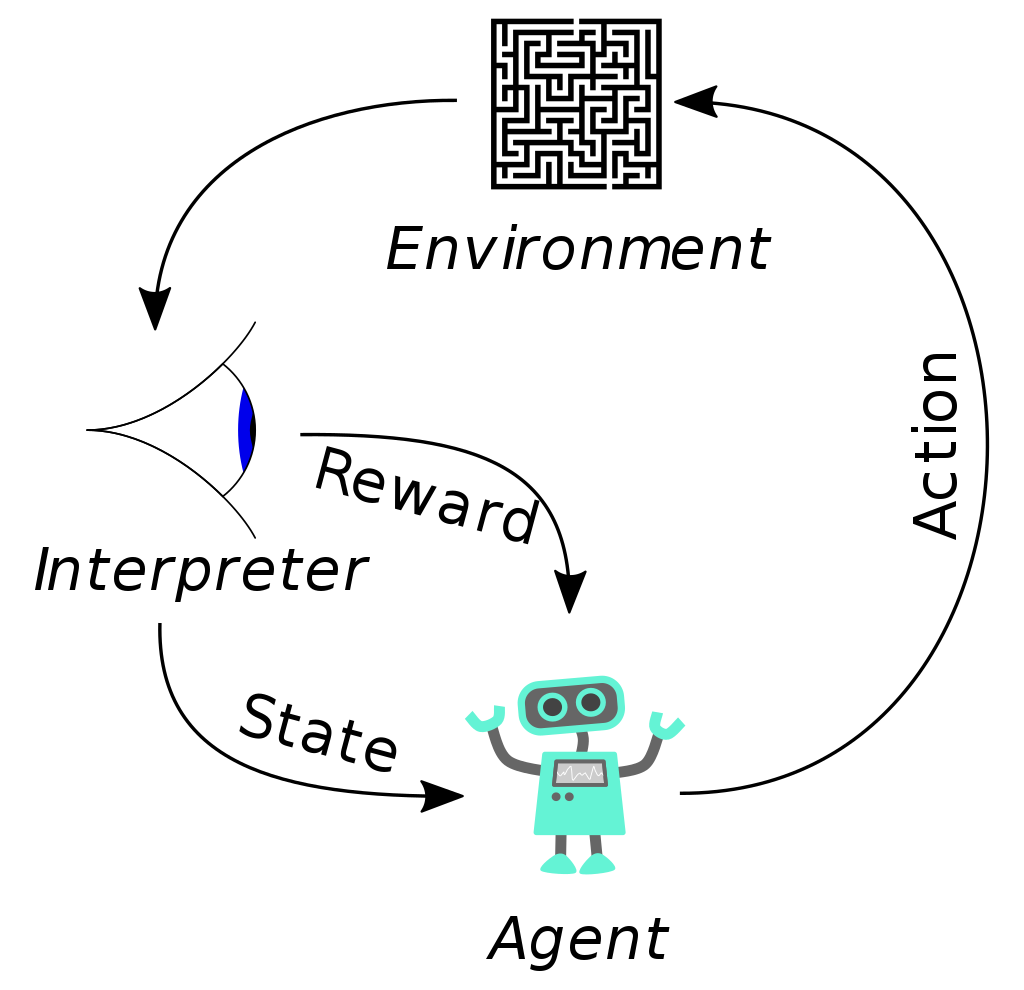
\includegraphics[width=7cm]{assets/rl_diagram.png}}
    \caption{Ciklus interakcije agenta s okolinom - TODO ref}
    \label{fig:rl}
\end{figure}

\section{Duboki modeli}

Duboko učenje \engl{Deep learning} jest tip strojnog učenja (točnije, podskup strojnog učenja) koje nastoji oponašati način zaključivanja i obrasce koje ljudski mozak koristi za učenje i donošenje odluka. Veliku ulogu u cijeloj ideji dubokog učenja imaju duboke neuronske mreže \engl{deep neural networks, DNN} pomoću kojih se povezivanjem više slojeva procesnih elemenata (čvorova, neurona), dobivaju duboki modeli koji su sposobni učiti i baratati s podatcima kompozitne strukture. Primjenom dubokih modela dolazimo do slijeda naučenih nelinearnih transformacija kojima aproksimiramo funkciju odluke, učimo mapiranje između ulaznih podataka i izlazih podataka, te nastojimo postići dobru generalizaciju nad stvarnim podatcima. 

\subsection{Unaprijedni potpuno povezani modeli}

Unaprijedni potpuno povezani modeli \engl{Fully connected neural network} (poznatiji i pod nazivom višeslojni perceptron \engl{Multi-layer perceptron}) sastoje se od lanaca potpuno povezanih slojeva. Svaki neuron iz prethodnog sloja povezan je s neuronom idućeg sloja. 

Sastoje se od tri vrste slojeva - ulaznog sloja, izlaznog sloja i skrivenih slojeva. Ulaznom sloju dovode se podatci koje je potrebno obraditi. Izlaz neuronske mreže (u najosnovnijem obliku) predstavljen je logitima \engl{logits} - vektorima logaritama nenormaliziranih vrijednosti. Specifičnije, za slučaj da želimo provesti klasifikaciju podataka ili drugačije organizirati izlazne vrijednosti na izlaz dodajemo posebni sloj (npr. \textit{Softmax} funkcija za klasifikaciju). Samo su ulaz i izlaz specificirani dimenzijama. Model ima slobodu da iskoristi skrivene slojeve na način koji osigurava najbolju aproksimaciju funkcije. Neuronskim mrežama želimo izgraditi modele koji nisu linearno odvojivi i zato koristimo nelinearnu aktivacijsku funkciju - najčešće ReLU (Rectified Linear Unit). Svaki od slojeva modelira jednu nelinearnu transformaciju.

Slika \ref{fig:nn} \cite{NNsvg} prikazuje arhitekturu potpuno povezanog modela koji je sastavljen od sveukupno 4 potpuno povezana sloja - ulaznog (dimenzije 4), izlaznog (dimenzije 2) i dva skrivena sloja (svaki dimenzije 8). Kodom \ref{lst:fcn} prikazana je implementacija navedenog modela u biblioteci \textit{PyTorch}.

\begin{figure}[H]
    \centering
    \frame{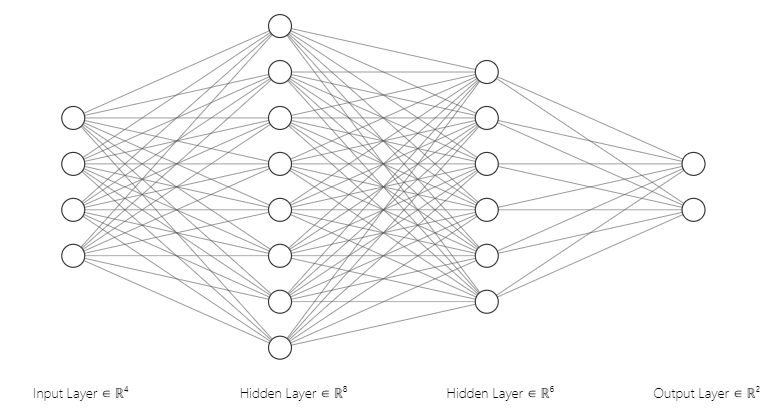
\includegraphics[width=11cm]{assets/nn.png}}
    \caption{Arhitektura potpuno povezanog modela}
    \label{fig:nn}
\end{figure}

\begin{listing}[H]
    \caption{Implementacija potpuno povezanog modela na slici \ref{fig:nn} koristeći biblioteku \textit{PyTorch}}
    \inputminted{python}{snippets/fcn.py}
    \label{lst:fcn}
\end{listing}

\subsection{Konvolucijski modeli}

Konvolucijski modeli \engl{Convolutional neural networks} su modeli koji uz potpuno povezane slojeve imaju najmanje jedan konvolucijski sloj \engl{convolution layer}. Osim spomenutih slojeva, konvolucijski modeli sadrže i slojeve sažimanja \engl{pooling layers}, slojeve u kojima provodimo nelinearnost podataka te sloj koji višedimenzionalni ulaz pretvara u jednodimenzionalni i pritom priprema podatke za obradu u potpuno povezanim slojevima \engl{flatten layer}.

Operacija konvolucije provodi se nad ulazom i jezgrom \engl{kernel} (slobodnim parametrima koje učimo) gdje kao rezultat dobivamo mapu značajki koja pokazuje gdje se koja značajka nalazi u ulaznim podatcima (npr. slici). Dimenzije mapa značajki i njihovu robusnost korigiramo korištenjem atributa koraka konvolucije \engl{stride} i nadopunjavanja ulaznih podataka \engl{padding}. Slično konvolucijskom sloju, sloj sažimanja odgovoran je za smanjenje prostora značajki (smanjenje dimenzionalnosti podataka) i dodatno za izdvajanje dominantnih značajki. Razlikujemo dvije vrste sažimanja: sažimanje maksimalnom vrijednosti \engl{max pooling} i sažimanje srednjom vrijednosti \engl{average pooling}. Prilikom sažimanja značajki maksimalnom vrijednošću u obzir uzimamo samo značajku najveće vrijednosti te na taj način uklanjamo šum ulaza i potencijalno biramo značajku najveće važnosti.

Korištenje konvolucijskih modela biti će nam iznimno potrebno u situacijama kada su ulazni podatci u formi slike, odnosno kada su nam važne lokalne interakcije između ulaznih podataka (piksela) te njihova vremenska i prostorna ovisnost.

Slika \ref{fig:cnn} \cite{NNsvg} prikazuje jednostavni konvolucijski model koji se sastoji od konvolucijskog sloja, sloja sažimanja maksimalnom vrijednosti, sloja koji 3-dimenzionalne podatke pretvara u 1-dimenzionalne, te dva potpuno povezana sloja. Ulaz u konvolucijski sloj predstavlja RGB slika (3 kanala) dimenzije $32 \times 32$. Primjenom konvolucije (veličina jezgre 3, korak 3, nadopuna 1) izvlačimo 18 kanala značajki dimenzije $32 \times 32$ (dimenzija se nije promijenila iz razloga što nadopunjavamo ulaz). Primjenom sažimanja maksimumom (veličina jezgre 2, korak 2) smanjujemo broj značajki na dimenziju $16 \times 16$. Prvi potpuno povezani sloj na svoj ulaz dobije vektor dimenzije $4608$ kojeg pretvara u vektor izlaza dimenzije $64$. Posljednji potpuno povezani sloj koji je ujedno i posljednji sloj u ovom konvolucijskom modelu za izlaz predaje vektor dimenzije $10$. Isječak koda koji prikazuje implementaciju jednostavnog konvolucijskog modela koristeći bibilioteku \textit{PyTorch} prikazan je kodom \ref{lst:cnn}.

\begin{figure}[H]
    \centering
    \frame{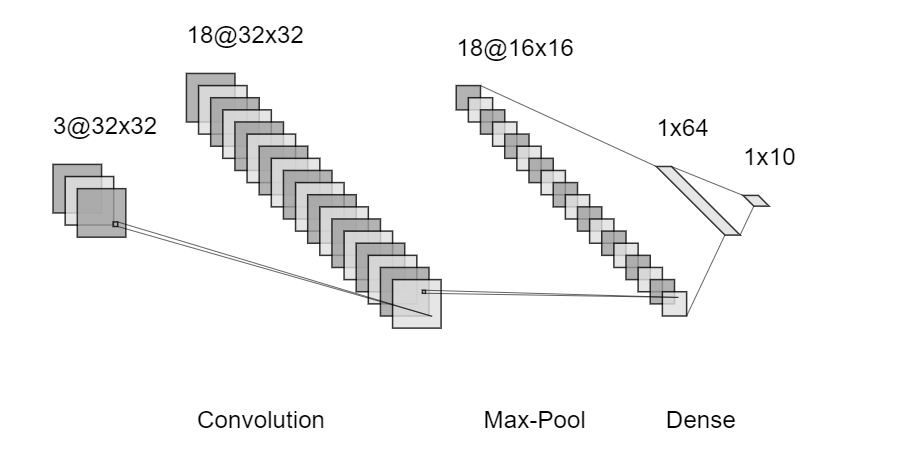
\includegraphics[width=11cm]{assets/cnn.png}}
    \caption{Arhitektura konvolucijskog modela}
    \label{fig:cnn}
\end{figure}

\begin{listing}[H]
    \caption{Implementacija konvolucijskog modela na slici \ref{fig:cnn} koristeći biblioteku \textit{PyTorch}}
    \inputminted{python}{snippets/cnn.py}
    \label{lst:cnn}
\end{listing}

\section{Algoritmi podržanog učenja}

Svaki model strojnog učenja definiran modelom, gubitkom i metodom optimizacije. Model je postupak obrade (odnosno skup funkcija) sa slobodnim parametrima koji za određen ulaz daje pripadajući izlaz. Gubitak je mjera koja na formaliziran način vrednuje slobodne parametre modela, odnosno pokazuje u kojoj mjeri se mi ne slažemo s onim što je model predstavio kao izlaz. Metoda optimizacije (optimizacijski postupak) jest način na koji pronalazimo optimalne parametre koji su važni kako bi minimizirali prethodno navedenu komponentu - gubitak. Navedene tri glavne komponente biti će važno napomenuti pri svakom predstavljaju algoritma jer su to glavne odrednice pri analizi algoritama strojnog učenja.

TODO dodati dio oko value functions, advantage functions... kako bi bilo kasnije lakše objasniti algoritme, funkcije gubitka, što koja mreža predstavlja...

% https://spinningup.openai.com/en/latest/spinningup/rl_intro2.html

% dodati literaturu https://www.fer.unizg.hr/_download/repository/SU-2020-02-OsnovniKoncepti.pdf

\subsection{Deep Q Learning}

TODO https://github.com/udacity/deep-learning/blob/master/reinforcement/nature14236.pdf

\subsection{Double Deep Q Learning}

TODO https://arxiv.org/pdf/1509.06461.pdf

\subsection{Actor Critic}

TODO https://www.tensorflow.org/tutorials/reinforcement_learning/actor_critic
